\documentclass[10pt,openany,a4paper]{article}
\usepackage{tikz, pgfplots, tkz-euclide,calc}
\usetikzlibrary{patterns,shapes.arrows,calc}
\usepackage{fancyhdr}
\usepackage{enumerate,enumitem}
\usepackage{cancel}
\usepackage{varwidth}

% TAMBAHKAN PACKAGE SENDIRI KALAU KURANG

\usepackage{geometry}
\geometry{
	left = 22mm,
	right = 22mm,
	top = 25mm,
	bottom = 25mm,
}
\usepackage{graphicx}
\usepackage{subcaption}
\usepackage{soul}
\usepackage{hyperref}
\usepackage{float}
\usepackage{setspace}
\usepackage{afterpage}
\usepackage{xcolor}
\usepackage[nosectionbib]{apacite}
\usepackage{lmodern}
\usepackage{mathtools}
\usepackage{upgreek}
\usepackage{siunitx}
\usepackage{physics}
\usepackage{hyperref}
\renewcommand{\baselinestretch}{1.3}
\usepackage{multicol}
\usepackage{hyperref,ragged2e,amsmath,multicol,gensymb,setspace,
fancyhdr,amsfonts,tikz,pgfplots,nccmath,enumerate,verbatim,amsthm,physics}
\usepgfplotslibrary{polar,fillbetween}
% Disable tikz externalization to avoid requiring -shell-escape
\usepgfplotslibrary{external}
\tikzexternalize[prefix=tikz/]
\tikzset{reuse path/.code={\pgfsyssoftpath@setcurrentpath{#1}}}
\usetikzlibrary{shapes.geometric,arrows}
\newcommand\mylog[1]{\mathop{{}^{#1}\mathrm{log}}}
\pgfplotsset{compat=1.15}
\pgfplotsset{my style/.append style={axis x line=middle, axis y line=
middle, xlabel={$x$}, ylabel={$y$}, axis equal }}
\usepackage{etoolbox}
% remove stray \makeatother
\newtheorem{defn}{Definisi}[section]
\newtheorem{teo}[defn]{Teorema}
\newtheorem{thm}{Teorema}[section]
\newtheorem{lemma}{Lemma}
\newtheorem{lemmas}[defn]{Lemma}
\newtheorem{cor}[defn]{Akibat}
\newtheorem{asumsi}[defn]{Asumsi}
\theoremstyle{definition}
\newtheorem{con}{Contoh}[section]
\theoremstyle{definition}
\theoremstyle{plain}
\newtheorem{prop}{Proposisi}[section]
\renewcommand{\proofname}{Bukti}
\renewcommand{\thethm}{\arabic{chapter}.\arabic{thm}}

\newcommand{\normlp}[1]{\left\|#1\right\|_{L^p_{\lambda}(0,T;H)}}% Fungsi norm (||x||)
\newcommand{\R}{\mathbb{R}}
\renewcommand{\natural}{\mathbb{N}}
\newcommand{\Xpl}{X^R_{p,\lambda}}
\newcommand{\Xpls}{X^R_{p,\lambda^*}}
\newcommand{\qpl}{q^R_{p,\lambda}}
\newcommand{\qpls}{q^R_{p,\lambda^*}}
\pagestyle{fancy}
\fancyhf{}
\lhead{Halaman \thepage}
\rhead{Pembahasan Soal ETS 2023/2024 \\ (\href{https://instagram.com/ahmadzakiyudin_/}{@ahmadzakiyudin\_})}
\hypersetup{
    colorlinks=true,
    linkcolor=blue,
    filecolor=blue,      
    urlcolor=blue,
}
\newenvironment{jawab}[2][tes]{
% \fbox{\begin{minipage}{14.65cm}
\textbf{Kata kunci materi:} #1.\\
\textbf{Penyelesaian:} #2
% \end{minipage}}
}{}

\newenvironment{jawab2}[2][tes]{
\fbox{\begin{minipage}{14.65cm}
 #2
\end{minipage}}}{}

\newenvironment{jawaban}[2][tes]{
\colorlet{oldcolor}{.}
        \color{red}
        \setlength{\fboxrule}{1pt}\boxed{\color{oldcolor}#2}\color{oldcolor}.
}{}

\newenvironment{jawaban2}[2][tes]{
\colorlet{oldcolor}{.}
        \color{red}
        \setlength{\fboxrule}{1pt}\fbox{\color{oldcolor}#2}\color{oldcolor}.
}{}

\newenvironment{penting}[2][tes]{
\colorlet{oldcolor}{.}
\color{blue}
\fbox{\color{oldcolor}#2}\color{oldcolor}
}{}

\begin{document}
\setlength\fboxsep{3pt}
% ensure enough header height for fancyhdr
\setlength{\headheight}{24pt}
\begin{enumerate}
     \item Dapatkan luas permukaan yang dibentuk oleh perputaran kurva $x=3-y$ dari $y=0$ sd $y=2$ diputar terhadap sumbu-$y$. Sketsa kurva tersebut. \\
     \begin{jawab}[luas permukaan benda putar, grafik fungsi, integral tentu, turunan]{\\
        Berikut adalah sketsa dari kurva $x=3-y$ untuk $y$ dari 0 hingga 2, yang diputar terhadap sumbu-$y$ untuk membentuk sebuah benda putar.
    \begin{center} 
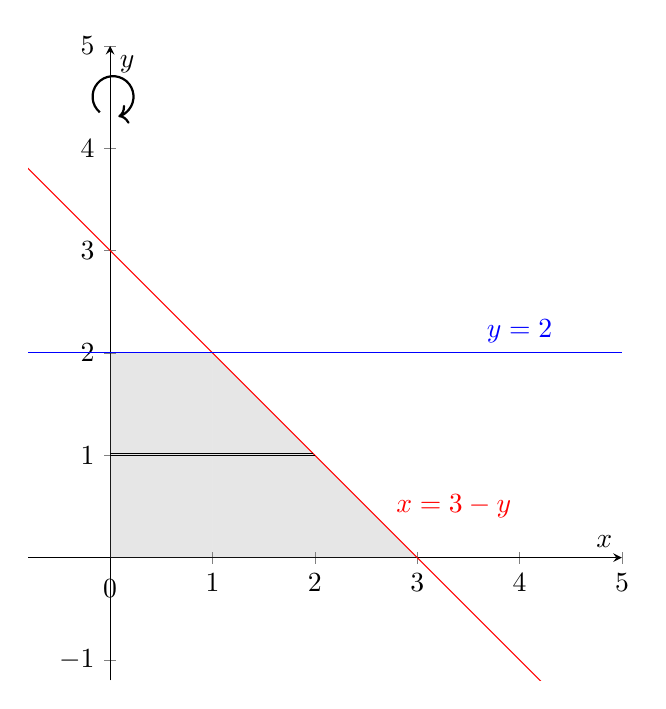
\begin{tikzpicture}
\begin{axis}[
x =1.3 cm, y=1.3 cm,
axis lines=middle,
xmin=-0.8,xmax=5,
ymin=-1.2,ymax=5,
xtick distance=1,
ytick distance=1,
xlabel=$x$,
ylabel=$y$
]

% Kurva y = 3-x
\addplot [red,domain=1:3, samples=1000, name path=A] {3-x};
\addplot [red,domain=-1:1, samples=1000] {3-x};
\addplot [red, domain=3:5, samples=1000]{3-x};

\addplot [opacity=0,domain=1:3,name path=B] {0};
\addplot [blue,domain=-1:0] {2};
\addplot [blue,domain=1:5] {2};
\addplot [blue,domain=0:1,name path=C] {2};
\addplot [opacity=0,domain=0:1,name path=D] {0};

% Daerah arsiran
\addplot[gray,opacity=0.2] fill between[of=A and B, soft clip={domain=1:3}];
\addplot[gray,opacity=0.2] fill between[of=C and D, soft clip={domain=0:1}];

    % Node garis x=3-y
    \draw[red] (2.7,0.5) node[right] {$x=3-y$};
    %Node garis y=2
    \draw[blue] (4,2) node[above] {$y=2$};

% Partisi
\draw (0,1) -- (3-1,1);
\draw (0,1.015) -- (3-1.015,1.015);

% %Penanda jari-jari luar
% \draw[dashed,<->] (2.7,2*2.7-2) -- (2.7,0);
% \draw (2.7,1.5) node[right] {$r_l$};

% %Penanda jari-jari dalam
% \draw[dashed,<->] (2.2,-2*2.2+6) -- (2.2,0);
% \draw (2.2,0.7) node[left] {$r_d$};

% Label x=0
\draw (0,-0.3) node{$0$};
\draw[thick,->]
(-0.1,4.35)
arc[start angle=230,end angle=-75,radius=0.2];
\end{axis}
\end{tikzpicture}
\end{center}
Diperhatikan bahwa luas permukaan yang dibentuk oleh perputaran kurva $x=g(y)$ dari $y=a$ hingga $y=b$ diputar terhadap sumbu-$y$ dapat dihitung menggunakan rumus berikut:
\begin{align*}
    S &= 2\pi \int_{a}^{b} g(y) \sqrt{1 + \left(g'(y)\right)^2} dy
    \end{align*}
Dalam hal ini $g(y) = 3-y$ sehingga $g'(y) = -1$. Batas integralnya adalah $a=0$ dan $b=2$. Kemudian, kita dapat menghitung luas permukaan sebagai berikut:
\begin{align*}
    S &= 2\pi \int_{0}^{2} (3-y) \sqrt{1 + (-1)^2} dy \\
    &= 2\pi \int_{0}^{2} (3-y) \sqrt{2} dy \\
    &= 2\pi \sqrt{2} \int_{0}^{2} (3-y) dy \\
    &= 2\pi \sqrt{2} \left[ 3y - \frac{y^2}{2} \right]_{0}^{2} \\
    &= 2\pi \sqrt{2} \left[ 6 - 2 \right] \\
    &= 8\pi \sqrt{2}
\end{align*}
      }
    \end{jawab}
      \item Dapatkan volume benda padat yang diperoleh dari daerah yang dibatasi $y=2x-2,y=-2x+6,x=3$ diputar pada sumbu-$x$ (Sketsa bidang datar dan sumbu putarnya seperti gambar di bawah ini).\\
      \begin{jawab}[volume benda putar, metode cakram, grafik fungsi, integral tentu]{
        \\
            Untuk menggambar kurvanya, kita perlu mencari titik potong antara kurva $y=2x-2$ dan $y=-2x+6$ dengan menyamakan kedua persamaan tersebut:
\begin{align*}
2x - 2 = -2x + 6 \qquad \Longleftrightarrow \qquad 4x = 8 \qquad \Longleftrightarrow \qquad x = 2
\end{align*}
Kemudian, dengan mensubstitusi $x=2$ ke salah satu persamaan, misalnya $y=2x-2$, kita dapatkan nilai $y=2(2)-2=4-2=2$.
Jadi, titik potong antara kedua kurva tersebut adalah $(2, 2)$. Berikut ini adalah sketsa dari kurva $y=2x-2$ dan $y=-2x+6$ yang dibatasi oleh garis vertikal $x=3$, serta sumbu-$x$ sebagai sumbu putarnya.
    \begin{center} 
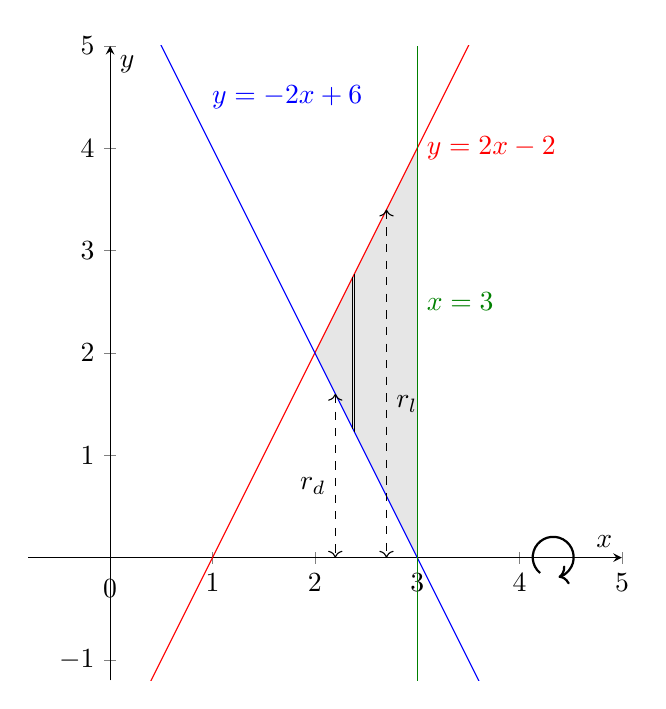
\begin{tikzpicture}
\begin{axis}[
x =1.3 cm, y=1.3 cm,
axis lines=middle,
xmin=-0.8,xmax=5,
ymin=-1.2,ymax=5,
xtick distance=1,
ytick distance=1,
xlabel=$x$,
ylabel=$y$
]

% Kurva y = 2x-2 
\addplot [red,domain=2:3, samples=1000, name path=A] {2*x-2};
\addplot [red,domain=-1:2, samples=1000] {2*x-2};
\addplot [red,domain=3:6, samples=1000] {2*x-2};

% Kurva y = -2x + 6
\addplot [blue,domain=2:3, samples=1000,name path=B] {-2*x+6};
\addplot [blue,domain=-1:2, samples=1000] {-2*x+6}; 
\addplot [blue,domain=3:6, samples=1000] {-2*x+6}; 

% Daerah arsiran
\addplot[gray,opacity=0.2] fill between[of=A and B, soft clip={domain=0:4}];

% Garis x = 3
\draw[green!50!black] (3,-1.4) -- (3,5);

% Node garis x = 3
\draw[green!50!black] (3,2.5) node[right] {$x=3$};
%Node kurva y = 2x - 2
\draw[red] (3,4) node[right] {$y=2x-2$};
%Node kurva y = -2x + 6
\draw[blue] (0.9,4.5) node[right] {$y=-2x+6$};

% Partisi
\draw (2.37,2*2.37-2) -- (2.37,-2*2.37+6);
\draw (2.385,2*2.385-2) -- (2.385,-2*2.385+6);

%Penanda jari-jari luar
\draw[dashed,<->] (2.7,2*2.7-2) -- (2.7,0);
\draw (2.7,1.5) node[right] {$r_l$};

%Penanda jari-jari dalam
\draw[dashed,<->] (2.2,-2*2.2+6) -- (2.2,0);
\draw (2.2,0.7) node[left] {$r_d$};

% Label x=0
\draw (0,-0.3) node{$0$};
\draw[thick,->]
(4.2,-0.15)
arc[start angle=230,end angle=-75,radius=0.2];
\end{axis}
\end{tikzpicture}

\end{center}
Diperhatikan bahwa batas atas dan batas bawah daerah tersebut dari $x=2$ hingga $x=3$ selalu sama, yaitu batas atas $y=2x-2$ dan batas bawah $y=-2x+6$. Oleh karena itu, akan lebih mudah jika kita dapat mengambil partisi yang tegak lurus dengan sumbu putar, yaitu garis vertikal yang memotong daerah tersebut. \\
Didapatkan bahwa jari-jari luar $r_l$ adalah jarak dari sumbu putar ke kurva $y=2x-2$, sedangkan jari-jari dalam $r_d$ adalah jarak dari sumbu putar ke kurva $y=-2x+6$. Karena sumbu putarnya adalah sumbu-$x$, maka didapatkan bahwa $r_l = 2x-2$ dan $r_d = -2x+6$. Kemudian, kita dapat menghitung volume benda padat yang diperoleh dari perputaran daerah tersebut menggunakan metode cakram sebagai berikut:
\allowdisplaybreaks
\begin{align*}
    V &= \pi \int_{a}^{b} \left( r_l^2 - r_d^2 \right) dx\\
    &= \pi \int_{2}^{3} \left( r_l^2 - r_d^2 \right) dx \\
    &= \pi \int_{2}^{3} \left( (2x-2)^2 - (-2x+6)^2 \right) dx \\
    &= \pi \int_{2}^{3} \left(4x^2 - 8x + 4 - (4x^2 - 24x + 36) \right) dx \\
    &= \pi \int_{2}^{3} \left(16x - 32\right) dx \\
    &= \pi \left[ 8x^2 - 32x \right]_{2}^{3} \\
    &= \pi \left[ (8\cdot 3^2 - 32\cdot 3) - (8\cdot 2^2 - 32\cdot 2) \right] \\
    &= \pi \left[ (72 - 96) - (32 - 64) \right] \\
    &= \pi \left[ -24 + 32 \right] \\
    &= 8\pi.
    \end{align*}   
      }
    \end{jawab}
        \item[3.] Tentukan luas daerah di dalam lingkaran $r=6$ dan di dalam kardioda $r=4+4\cos\theta$. Sketsa luasan bidang datar.\\
        \begin{jawab}[grafik fungsi polar, integral fungsi trigonometri, luas daerah di dalam kurva polar]{
             \\
             Untuk menggambar kurvanya, kita perlu mencari titik potong antara kurva $r=6$ dan $r=4+4\cos\theta$ dengan menyamakan kedua persamaan tersebut:
\begin{align*}
6 = 4 + 4\cos\theta \qquad \Longleftrightarrow \qquad 4\cos\theta = 2 \qquad \Longleftrightarrow \qquad \cos\theta = \frac{1}{2}
\end{align*}
Kemudian, kita dapatkan nilai $\theta$ sebagai berikut:
\begin{align*}
\theta = \pm \frac{\pi}{3} + 2k\pi, \quad k \in \mathbb{Z}
\end{align*}
Jadi, titik potong antara kedua kurva tersebut terjadi pada $\theta = \frac{\pi}{3}$ dan $\theta = -\frac{\pi}{3}$. Berikut ini adalah sketsa dari kedua kurva tersebut, yaitu lingkaran $r=6$ dan kardioda $r=4+4\cos\theta$, serta daerah yang diarsir yang merupakan daerah di dalam kedua kurva tersebut.
    \begin{center}
        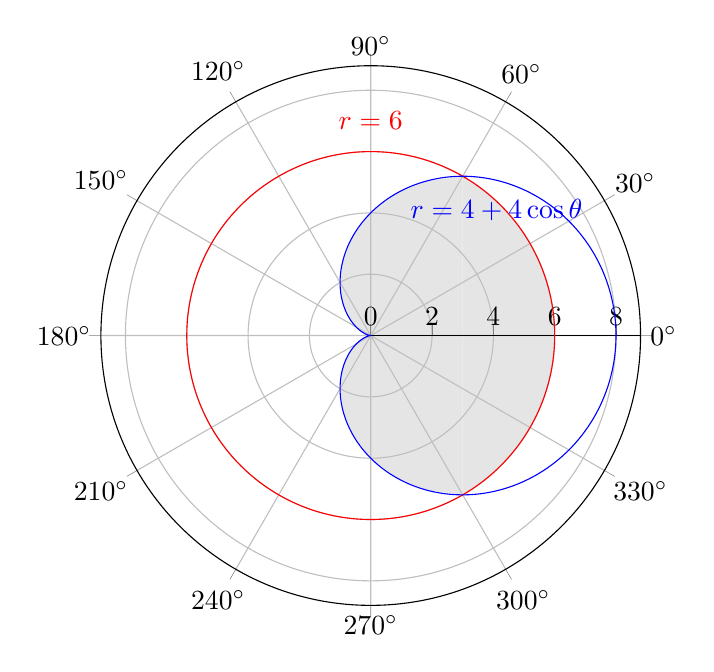
\begin{tikzpicture}
\pgfplotsset{set layers}
  \begin{polaraxis}[xticklabel={$ \pgfmathprintnumber{\tick}^{\circ} $}]
    \addplot[domain=0:360,samples=300, color=red] {6};
    \addplot[domain=-60:60,opacity=0, save path=\A] {6};
    \addplot[domain=60:300,opacity=0, save path=\B] {4+4*cos(x)};
    %Node kurva r=6
    \node[red] at (axis cs:90,7) {$r=6$};
    %Node kurva r=4+4*cos(x)
    \node[blue] at (axis cs:45,5.8) {$r=4+4\cos\theta$};
    \pgfonlayer{axis background}
    \fill[gray!20, reuse path=\A];
    \fill[gray!20, reuse path=\B];
    \endpgfonlayer
    \addplot[domain=0:360,samples=300, color=blue] {4+4*cos(x)};
  \end{polaraxis}

  \end{tikzpicture}
    \end{center}
%   \begin{center}
% 	\begin{tikzpicture}
% \begin{axis}[
% x= 1 cm, y=1 cm,
%  axis lines=middle,
%   xmin=-0.8,xmax=5,ymin=-0.5,ymax=3,
%   xtick={0},
%   ytick={0},
%   xlabel=$x$,
%   ylabel=$y$]
% \addplot [domain=0:1,samples=3000] {sqrt(4-4*x)};
% \draw (1,-0.03) node[below] {$a$};
% \draw (-0.03,2) node[left] {$2a$};
% \addplot[domain=0:90,samples=300,data cs=polar] (x,{4+4*cos(x)});
% \draw (4,-0.03) node[below] {$4a$};
% \end{axis}
% \end{tikzpicture}
% \end{center}
Diperhatikan bahwa daerah tersebut simetri terhadap sumbu-$x$, sehingga kita dapat menghitung luas daerah tersebut dengan menghitung luas daerah di atas sumbu-$x$ dan kemudian mengalikannya dengan 2. \\
Diperhatikan pula bahwa daerah di atas sumbu-$x$ dibatasi oleh kurva $r=6$ untuk $\theta$ dari $0$ hingga $\frac{\pi}{3}$, dan dibatasi oleh kurva $r=4+4\cos\theta$ untuk $\theta$ dari $\frac{\pi}{3}$ hingga $\pi$. Berikut adalah visualisasi dari daerah yang akan dihitung luasnya:
    \begin{center}
        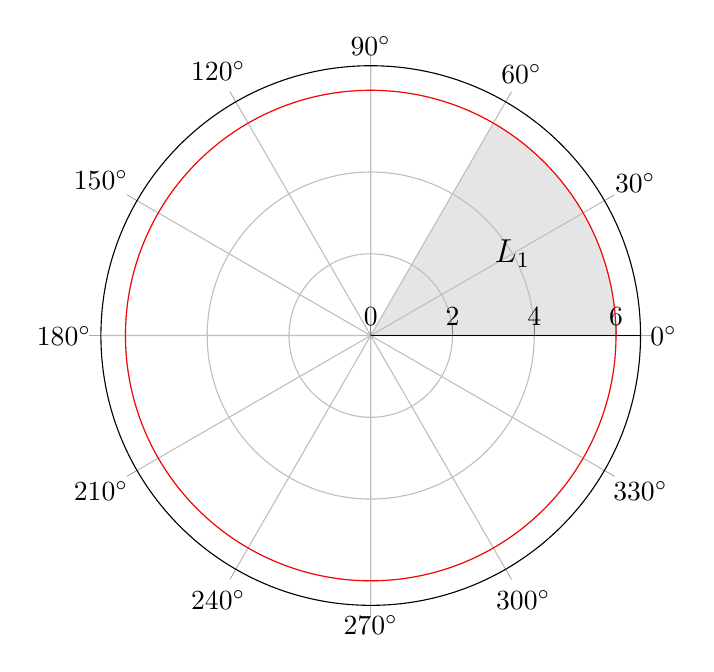
\begin{tikzpicture}
\pgfplotsset{set layers}
  \begin{polaraxis}[xticklabel={$ \pgfmathprintnumber{\tick}^{\circ} $}]
    \addplot[domain=0:360,samples=300, color=red] {6};
    \node at (axis cs:30,4) {\large{$L_1$}};
    \addplot[domain=0:60,opacity=0, save path=\apa] {6} -- (axis cs:60,0)
-- (axis cs:0,0)
-- cycle;
    \pgfonlayer{axis background}
    \fill[gray!20, even odd rule, reuse path=\apa];
    \endpgfonlayer
    % \addplot[domain=0:360,samples=300, color=blue] {4+4*cos(x)};
  \end{polaraxis}
    \end{tikzpicture}
    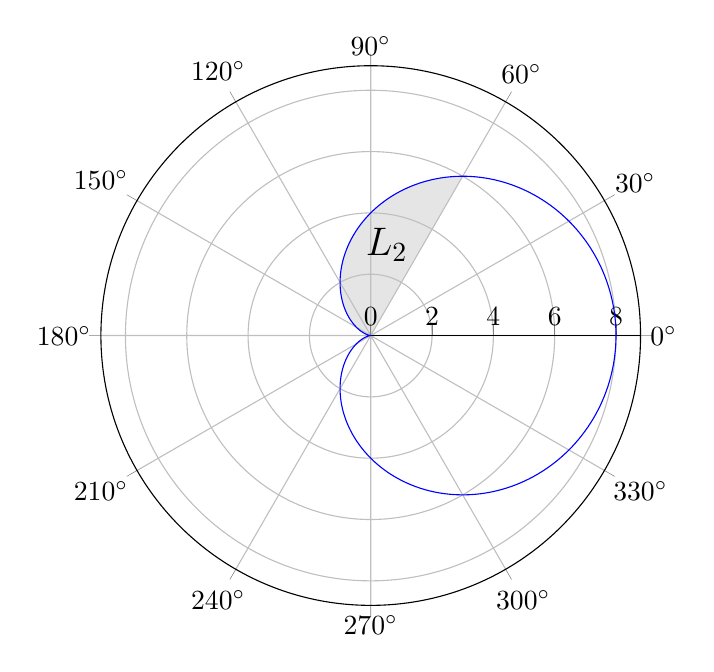
\begin{tikzpicture}
\pgfplotsset{set layers}
  \begin{polaraxis}[xticklabel={$ \pgfmathprintnumber{\tick}^{\circ} $}]
    % \addplot[domain=0:360,samples=300, color=red] {6};
    \addplot[domain=60:180,opacity=0, save path=\B] {4+4*cos(x)};
    \node at (axis cs:80,3) {\Large{$L_2$}};
    \pgfonlayer{axis background}
    \fill[gray!20, reuse path=\B];
    \endpgfonlayer
    \addplot[domain=0:360,samples=300, color=blue] {4+4*cos(x)};
  \end{polaraxis}
    \end{tikzpicture}
    \end{center}
    Ingat kembali bahwa luas daerah yang dibatasi oleh kurva polar $r=f(\theta)$ dari $\theta=a$ hingga $\theta=b$ dapat dihitung menggunakan rumus berikut:
\begin{align*}
A = \frac{1}{2} \int_{a}^{b} f(\theta)^2 d\theta
\end{align*}
Dengan menggunakan rumus tersebut, didapatkan luas daerah $L_1$ yang dibatasi oleh kurva $r=6$ untuk $\theta$ dari $0$ hingga $\frac{\pi}{3}$ sebagai berikut:
\allowdisplaybreaks
\begin{align*}
L_1 &= \frac{1}{2} \int_{0}^{\frac{\pi}{3}} 6^2 d\theta \\
&= \frac{1}{2} \int_{0}^{\frac{\pi}{3}} 36 d\theta \\
&= 18 \int_{0}^{\frac{\pi}{3}} d\theta \\
&= 18 \left[ \theta \right]_{0}^{\frac{\pi}{3}} \\
&= 18 \cdot \frac{\pi}{3} \\
&= 6\pi
\end{align*}
Selanjutnya, didapatkan luas daerah $L_2$ yang dibatasi oleh kurva $r=4+4\cos\theta$ untuk $\theta$ dari $\frac{\pi}{3}$ hingga $\pi$ sebagai berikut:
\allowdisplaybreaks
\begin{align*}
L_2 &= \frac{1}{2} \int_{\frac{\pi}{3}}^{\pi} (4+4\cos\theta)^2 d\theta \\
&= \frac{1}{2} \int_{\frac{\pi}{3}}^{\pi} (16 + 32\cos\theta + 16\cos^2\theta) d\theta \\
&= \frac{1}{2} \int_{\frac{\pi}{3}}^{\pi} (16 + 32\cos\theta + 16\cdot\frac{1+\cos(2\theta)}{2}) d\theta \\
&= \frac{1}{2} \int_{\frac{\pi}{3}}^{\pi} (16 + 32\cos\theta + 8 + 8\cos(2\theta)) d\theta \\
&= \frac{1}{2} \int_{\frac{\pi}{3}}^{\pi} (24 + 32\cos\theta + 8\cos(2\theta)) d\theta \\
&= \frac{1}{2} \left[ 24\theta + 32\sin\theta + 4\sin(2\theta) \right]_{\frac{\pi}{3}}^{\pi} \\
&= \frac{1}{2} \left[ (24\pi + 32\sin\pi + 4\sin(2\pi)) - (24\cdot\frac{\pi}{3} + 32\sin\frac{\pi}{3} + 4\sin\frac{2\pi}{3}) \right] \\
&= \frac{1}{2} \left[ 24\pi - (8\pi + 32\cdot\frac{\sqrt{3}}{2} + 4\cdot\frac{\sqrt{3}}{2}) \right] \\
&= \frac{1}{2} \left[ 24\pi - 8\pi - 16\sqrt{3} - 2\sqrt{3} \right] \\
&= \frac{1}{2} \left[ 16\pi - 18\sqrt{3} \right] \\
&= 8\pi - 9\sqrt{3}
\end{align*}
Jadi, luas daerah yang di dalam kedua kurva tersebut adalah dua kali $L_1 + L_2$ sebagai berikut:
\begin{align*}
A &= 2(L_1 + L_2) \\
&= 2(6\pi + 8\pi - 9\sqrt{3}) \\
&= 2(14\pi - 9\sqrt{3}) \\
&= 28\pi - 18\sqrt{3}
\end{align*}
        }
        \end{jawab}
    

        \item[4.] Diberikan persamaan parametrik: $x=3\cos t+2, ~y=3\sin t$
        \begin{enumerate}
            \item Dapatkan $\frac{dx}{dt},\frac{dy}{dt}$, dan $\frac{dy}{dx}$
            \item Dapatkan persamaan garis singgung di titik $t=\frac{\pi}{3}$
        \end{enumerate}
        \begin{jawab}
            [persamaan parametrik, turunan, persamaan garis]
            {
                \begin{enumerate}
                    \item Diperhatikan bahwa 
                    \begin{align*}
                        \frac{dx}{dt} &= -3\sin t \\
                        \frac{dy}{dt} &= 3\cos t \\
                        \frac{dy}{dx} &= \frac{\frac{dy}{dt}}{\frac{dx}{dt}} = \frac{3\cos t}{-3\sin t} = -\cot t
                    \end{align*}
                    \item Pada $t=\frac{\pi}{3}$, kita dapatkan titiknya sebagai berikut:
                    \begin{align*}
                        x\left(\frac{\pi}{3}\right) &= 3\cos\left(\frac{\pi}{3}\right) + 2 = 3\cdot\frac{1}{2} + 2 = \frac{7}{2} \\
                        y\left(\frac{\pi}{3}\right) &= 3\sin\left(\frac{\pi}{3}\right) = 3\cdot\frac{\sqrt{3}}{2} = \frac{3\sqrt{3}}{2}
                    \end{align*}
                    Kemudian, kita hitung gradien garis singgung pada $t=\frac{\pi}{3}$:
                    \begin{align*}
                        m &= \frac{dy}{dx}\bigg|_{t=\frac{\pi}{3}} = -\cot\left(\frac{\pi}{3}\right) = -\frac{1}{\sqrt{3}}
                    \end{align*}
                    Dengan titik $(\frac{7}{2}, \frac{3\sqrt{3}}{2})$ dan gradien $m$, kita dapatkan persamaan garis singgung menggunakan rumus titik-slope:
                    \begin{align*}
                        y - \frac{3\sqrt{3}}{2} &= -\frac{1}{\sqrt{3}}\left(x - \frac{7}{2}\right) 
                    \end{align*}
                \end{enumerate}
            }
        \end{jawab}
    

        \item[5.]  Uraikan deret di bawah ini sampai dengan lima suku pertama:
        \begin{align*}
            \sum_{n=1}^{\infty}\frac{n!}{5+n}
        \end{align*}
        Gunakan uji Rasio untuk menentukan konvergen atau divergen dari deret tersebut.\\
        \begin{jawab}
            [deret, uji rasio]{\\
                Misalkan $a_n = \frac{n!}{5+n}$. Maka, lima suku pertama dari deret tersebut dapat dihitung sebagai berikut:
                \begin{align*}
                    a_1 &= \frac{1!}{5+1} = \frac{1}{6} \\
                    a_2 &= \frac{2!}{5+2} = \frac{2}{7} \\
                    a_3 &= \frac{3!}{5+3} = \frac{6}{8} = \frac{3}{4} \\
                    a_4 &= \frac{4!}{5+4} = \frac{24}{9} \\
                    a_5 &= \frac{5!}{5+5} = \frac{120}{10} = 12
                \end{align*}
                % \begin{align*}
                %     S_1 &= a_1 = \frac{1!}{5+1} = \frac{1}{6} \\
                %     S_2 &= S_1 + a_2 = \frac{1}{6} + \frac{2!}{5+2} = \frac{19}{42} \\
                %     S_3 &= S_2 + a_3 = \frac{19}{42} + \frac{3!}{5+3} = \frac{101}{84} \\
                %     S_4 &= S_3 + a_4 = \frac{101}{84} + \frac{4!}{5+4} = \frac{325}{84} \\
                %     S_5 &= S_4 + a_5 = \frac{325}{84} + \frac{5!}{5+5} = \frac{1333}{84}
                % \end{align*}
                Jadi, lima suku pertama dari deret tersebut adalah $\frac{1}{6}, \frac{2}{7}, \frac{3}{4}, \frac{24}{9}, 12$.

                Selanjutnya, kita gunakan uji rasio untuk menentukan konvergensi atau divergensi dari deret tersebut. Uji rasio menyatakan bahwa jika
                \begin{align*}
                    L = \lim_{n\to\infty} \left|\frac{a_{n+1}}{a_n}\right|
                \end{align*}
                maka:
                Jika $L < 1$, deret konvergen.
                Jika $L > 1$, deret divergen.
                Jika $L = 1$, uji tidak menentukan.

                Didapatkan bahwa
                \allowdisplaybreaks
                \begin{align*}
                    L = \lim_{n\to\infty} \left|\frac{\frac{(n+1)!}{5+(n+1)}}{\frac{n!}{5+n}}\right| 
                    &= \lim_{n\to\infty} \left|\frac{(n+1)! (5+n)}{n! (5+(n+1))}\right| \\
                    &= \lim_{n\to\infty} \left|\frac{(n+1)(5+n)}{5+n+1}\right| \\
                    &= \lim_{n\to\infty} \frac{n^2+6n+5}{n+6} \\
                    &= \lim_{n\to\infty} \qty(n +\frac{5}{n+6})\\ 
                    &= \infty
                \end{align*}
                Karena $L = \infty > 1$, maka deret tersebut divergen.
            }
        \end{jawab}
    

\end{enumerate}
\end{document}


